\testCom
{%Номер задачи
	3.104
}
{%Условие
	условие
}
{%Дано
	дано
}
{%Найти
	найти
}
{%Решение
	%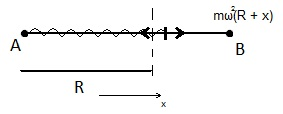
\includegraphics[height=30mm]{3_33.jpg}\\
	Очевидно, что $E_{мех} (t) = \frac{m x^2}{2} + \frac{k x^2}{2} = mgx,$ тогда средняя механическая энергия за период будет равна:\\
	$\frac{1}{T} \int\limits_0^T E_{мех}\, dt = \frac{\omega m}{2 \pi} \int\limits_0^{\frac{2 \pi}{\omega}} \left( \frac{x^2}{2} + \omega_0^2 \frac{x^2}{2} + gx \right)\, dt$\\
	Допустим, что $t \gg \frac{1}{\beta}$, т.е. x(t) = a $\cos (\omega t + \alpha)$ (а под интеграл можно внести  просто $x(t) = a \cos \omega t$, т.к. интегрируем по периоду):\\
	$\langle E_{мех} \rangle = \frac{\omega m}{4 \pi} \int\limits_0^{\frac{2 \pi}{\omega}} (\omega^2 a^2 \sin^2 \omega t + a^2 \omega_0^2 \cos^2 \omega t + \cancelto{0}{g \cos \omega t}\,\,) dt =$\\
 	$ = \frac{\cancel \omega m}{2 \cancel \pi} \frac{\cancel \pi a^2}{\cancel \omega} (\omega^2 + \omega_0^2) = m a^2 \frac{\omega^2 + \omega_0^2}{4}$\\
	(учли, что $\langle cos^2 \omega t \rangle = \langle \sin^2 \omega t \rangle = \frac{\pi}{\omega}$)\\
	
}

